\documentclass{article}
\usepackage{graphicx}
\usepackage[margin=1.5cm]{geometry}
\usepackage{amsmath}

\begin{document}
\twocolumn

\title{Monday warm-up: Kinematics, II}
\author{Prof. Jordan C. Hanson}

\maketitle

\section{Memory Bank}

\begin{enumerate}
\item $v = \frac{\Delta x}{\Delta t}$ ... Average velocity.
\item $v = \frac{dx}{dt}$ ... Instantaneous velocity.
\item $a = \frac{\Delta v}{\Delta t}$ ... Average acceleration.
\item $a = \frac{dv}{dt}$ ... Average acceleration.
\item $x(t) = \frac{1}{2}at^2 + v_i t + x_i$ ... Position versus time, given constant acceleration
\item $v(t) = at + v_i$ ... Speed versus time, given constant acceleration
\item $v_f^2 = v_i^2 + 2a\Delta x$ ... Initial and final speeds, given constant acceleration and displacement
\end{enumerate}

\section{Chapter 3 - Kinematics, II}

\begin{enumerate}
\item Suppose a runner accelerates at 3 m s$^{-2}$ from rest.  (a) \textit{Where} will the runner reach a top speed of 10 m s$^{-1}$? (b) \textit{When} does the runner reach top speed ? \\ \vspace{1.5cm}
\item Consider Fig. \ref{fig:graph}.  The formula that describes the speed of the system between 0 and 20 seconds is
\begin{itemize}
\item A: $v(t) = 3 t$
\item B: $v(t) = 0.3 t$
\item C: $v(t) = 20 t$
\item D: $v(t) = 0.2 t$
\end{itemize}
\item Using your formula for $v(t)$ from the previous exercise, what is the speed at $t = 10$ seconds? \\ \vspace{0.5cm}
\item Consider Fig. \ref{fig:graph}.  Between 50 and 70 seconds, the system
\begin{itemize}
\item A: has a positive acceleration
\item B: has a negative acceleration
\item C: has no acceleration
\item D: is not moving
\end{itemize}
\item Examine Fig. \ref{fig:graph}, and determine the regions with the largest positive acceleration and the largest negative acceleration.  Estimate them based on the graph. \\ \vspace{2cm}
\item The position of a system is $x(t)=5.0t^2 - 4.0t^3$ m. Find (a) the velocity and acceleration of the particle as functions of time, (b) the velocity and acceleration at t = 2.0 s, (c) the time at which the velocity is zero, and (d) the maximum position.
\end{enumerate}

\begin{figure}
\centering
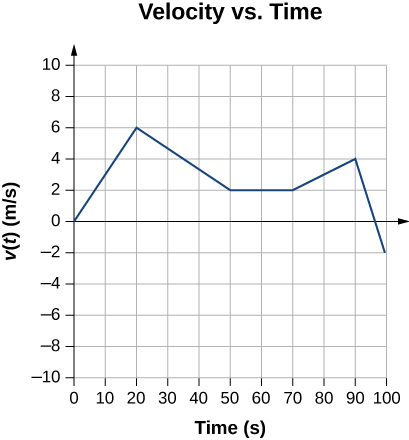
\includegraphics[width=0.35\textwidth]{figures/v_vs_t.jpeg}
\caption{\label{fig:graph} The velocity versus time for a system.}
\end{figure}

\end{document}
